\part{Approcci di risoluzione}

\begin{frame}
	\partpage
	\centering
\end{frame}

\begin{frame}
	\frametitle{Ricerca esaustiva}
	
	Approccio \textbf{Brute-force}:
	\begin{itemize}
		\item Enumerare tutti i $q$-path esistenti
		\item Contare le frequenze esatte di $f_A[w]$ e $f_B[w]$
		\item Calcolare la similarità usando la definizione
	\end{itemize}

	\pause
	\medskip
	
	Complessità:
	\begin{itemize}
		\item Tempo: $O(|V|^q)$
		\item Spazio: $O(|\Sigma|^q\ q)$
	\end{itemize}

	\pause
	\centering
	\medskip
	\textbf{Problema!}
	
	Limitare la ricerca mantenendo inalterato il valore di similarità
	
	\pause
	
	\begin{itemize}
		\item Tempo: $O(|V|^q)$ $\rightarrow$ Color Coding $\rightarrow$ $O(2^q\ |V|)$
		\item Spazio: $O(|\Sigma|^q\ q)$ $\rightarrow$ Sampling $\rightarrow$ $O(rq)$
	\end{itemize}
	
	
		
\end{frame}

\begin{frame}
	\frametitle{Color Coding}
	\centering

	\pause

		\begin{minipage}{.45\textwidth}
			\centering
			Coloriamo casualmente il grafo con $q$ colori e ci limitiamo ai path colorful 
			(percorsi con colori non ripetuti)
			\medskip
			
			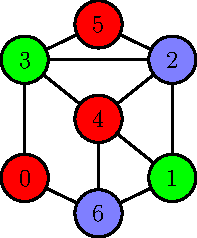
\includegraphics[width=0.5\textwidth]{images/8_cc_graph}
			
			\small
			\medskip
			
			Il numero dei path è esponenzialmente ridotto di un fattore $q! / q^q \simeq e^{-q}$\\
			 
			Per $q=3$ solo il $\sim22.22\%$\\
			Per $q=6$ solo il $\sim1.5\%$\phantom{$22$}
		\end{minipage}\hfill
		\pause
		\begin{minipage}{.45\textwidth}
			\centering
			
			\small
			
			$q!$ colorazioni accettabili\\
			$q^q$ possibili colorazioni
			
			\medskip
			
			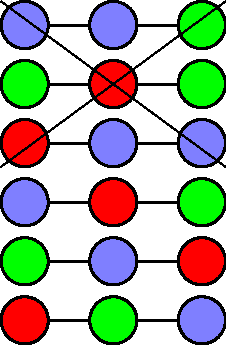
\includegraphics[width=0.5\textwidth]{images/8_cc_list}
			
			Esempi di possibili path\medskip
			
			In questo modo:
			\begin{equation*}
				f'_X[w] \simeq e^{-q} f_X[w]
			\end{equation*}
			\hfill
		\end{minipage}\hfill

\end{frame}

\begin{frame}
	\frametitle{Sampling}
	\centering
	
	\pause
	
	\begin{minipage}{.45\textwidth}
		\centering
		
		Tabella frequenze dei $q$-grammi: \medskip
		
		\begin{tabular}{|c|c|}
			\hline
			w   & $f_X[w]$  \\ \hline
			aaa &  721 \\ \hline
			abc &  243 \\ \hline
			... & ... \\ \hline
			zzy &   13 \\ \hline
			zzz &   368 \\ \hline
		\end{tabular}
	
		\medskip
		Potenzialmente:
		\medskip		 
		
		$|w| = |\Sigma|^q$ (tutti i $q$-grammi)
		\medskip		 
		 
		$\Sigma_w{f_X[w]} = |V|^q$ (tutti i $q$-path)
		
		
	\end{minipage}\hfill
	\pause
	\begin{minipage}{.45\textwidth}
		\centering
		Riduciamo le dimensioni della tabella \textbf{campionando uniformemente} $r$ colorful $q$-path distinti.\medskip
		
		Definiamo quindi:
		
		\begin{itemize}
			\item $R$ l'insieme dei $r$ $q$-path campionati ($r \ll |V|^q$ )
			\item $\mathcal{W}$ l'insieme dei $q$-grammi dei $q$-path in $R$ ($|W| \leq r$)
		\end{itemize}
		
		
		
		\hfill
	\end{minipage}\hfill

	\pause

	\bigskip
	
	\textbf{Jaccard}: campionamento con $X = A \cup B$
	
	\textbf{Bray-Curtis}: campionamento con $X = A \uplus B$
	
	
	
\end{frame}

\begin{frame}
	\frametitle{Esempio di sampling}
	\centering
	
	Campioniamo 5 diversi $3$-path da $X = A \cup B = \{ 0, 1, 12 \}$
	
	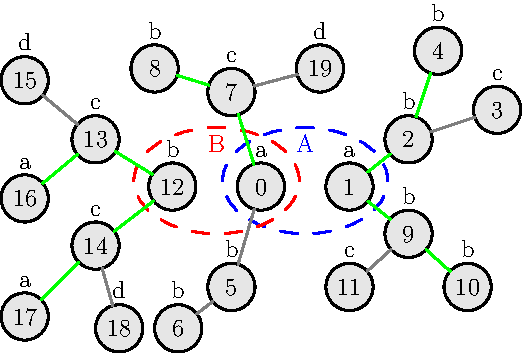
\includegraphics[width=0.5\textwidth]{images/13_sampl}
	
	\medskip
	
	R = \{ \color{green} 4-2-1 \color{darkgreen} 10-9-1  \color{green} 8-7-0 \color{darkgreen} 16-13-12  \color{green} 7-14-12 \color{black}\}
	
	$\mathcal{W} = $ \{ acb, bba, bca \}
	
	
\end{frame}

\begin{frame}
\frametitle{Approssimazione degli indici}
\centering

Dato un campione $\mathcal{W}$ di $q$-grammi 

approssimiamo i due indici limitandoci al campione

\pause

\begin{equation*}\label{jaccard-sub}	
J(A,B) = \frac{ \Sigma_{x \in \Sigma^{q}} \min(f_{A}[x], f_{B}[x]) }{ \Sigma_{x \in \Sigma^{q}} f_{A \cup B}[x] }
\end{equation*}
$\downarrow$
\begin{equation*}\label{jaccard-sub}	
J_{\mathcal{W}}(A,B) = \frac{ \Sigma_{x \in \mathcal{W}} \min(f_{A}[x], f_{B}[x]) }{ \Sigma_{x \in \mathcal{W}} f_{A \cup B}[x] }
\end{equation*}

\pause

\begin{equation*}\label{bray-sub}
BC(A,B) = \frac{ 2 \times \Sigma_{x \in \Sigma^{q}} \min(f_{A}[x], f_{B}[x]) }{ \Sigma_{x \in \Sigma^{q}} (f_{A}[x] + f_{B}[x]) }
\end{equation*}
$\downarrow$
\begin{equation*}\label{bray-sub}
BC_{\mathcal{W}}(A,B) = \frac{ 2 \times \Sigma_{x \in \mathcal{W}} \min(f_{A}[x], f_{B}[x]) }{ \Sigma_{x \in \mathcal{W}} (f_{A}[x] + f_{B}[x]) }
\end{equation*}

\end{frame}

\begin{frame}
	\frametitle{F-Count e F-Samp}
	\centering
	
	Come calcoliamo $f_A[w]$ e $f_B[w]$ per $w \in \mathcal{W}$?\medskip
	
	\pause
	
	\begin{minipage}{.45\textwidth}
		\centering
		\textbf{F-Count}
		
		Calcoliamo in modo esatto i valori di $f_A[w]$ e $f_B[w]$
		con una ricerca esaustiva limitata ai $q$-grammi in $\mathcal{W}$
		
		\bigskip
		
		\small		
		\textbf{Pro}:
		\begin{itemize}
			\item Più preciso in quanto usiamo le frequenze esatte
		\end{itemize}
		
		\textbf{Contro}:
		\begin{itemize}
			\item Potenzialmente lento in quanto potrebbe analizzare una grande porzione di grafo
		\end{itemize}
		
		\hfill
	\end{minipage}\hfill
	\pause
	\begin{minipage}{.45\textwidth}
		\centering
		\textbf{F-Samp}	
		
		 Stimiamo i valori di $f_A[w]$ e $f_B[w]$ 
		 usando il campione dei $q$-path $R$
		 
		 
		 \bigskip
		 
		 \small		
		 \textbf{Pro}:
		 \begin{itemize}
		 	\item Più veloce poichè analizziamo solo gli $r$ $q$-path campionati
		 \end{itemize}
		 
		 \textbf{Contro}:
		 \begin{itemize}
		 	\item Stima meno precisa dato che usiamo valori approssimati delle frequenze
		 \end{itemize}
		 
		\hfill
	\end{minipage}\hfill
	
\end{frame}

%\begin{frame}
%	\frametitle{Baseline}
%	\centering
%\end{frame}
